%%%%%%%%%%%%%%%%%%%%%%%%%%%%%%%%%%%%%%%%%%%%%%%%%%%%%%%%%%%%%%%%%%%%%%%%
\chapter{Ergebnisse}\label{sec:results}
%%%%%%%%%%%%%%%%%%%%%%%%%%%%%%%%%%%%%%%%%%%%%%%%%%%%%%%%%%%%%%%%%%%%%%%%

Dieser Teil der Arbeit beschäftigt sich mit den Ergebnissen der realisierten Applikation. Zuerst wird auf die einzelnen Iterationen eingegangen, die das Projekt während der Entstehung durchlaufen hat.
Die Entwicklung erfolgt iterativ, damit auf Änderungen der Anforderungen sofort reagiert werden kann und nicht am eigentlichen Ziel vorbei entwickelt wird. Zudem werden die Ergebnisse des Fragebogens evaluiert. Des Weiteren wird noch auf den Usability Aspekt der Applikation eingegangen. Daraufhin werden verschiedene Aspekte der theoretischen sowie praktischen Entwicklung näher beleuchtet.

\section{Iteration 1: Planung}\label{sec:iteration1}
In der Planungsphase wurden Therapeut/innen und Patient/innen gesucht, die sich bereit erklärten, an der Entwicklung der Applikation mitzuwirken. Das LK Allentsteig zeigte sich bereit, an der Entstehung der Applikation mitzuwirken. Um einen Einblick in den Therapiealltag zu erhalten und sich ein besseres Bild über die Behandlungsmöglichkeiten zu machen, wurde eine Führung durch das Haus vereinbart. Die Leitung stellte einen umfangreichen Zeitplan zusammen, der alle Stationen des Hauses umfasste. Zuerst fand ein Gespräch mit den leitenden Ärzt/innen statt, um etwaige Formalitäten für die Arbeit zu klären. Die Führung umfasste Einblicke in die Bereiche der Logopädie, Ergotherapie, Motorik und Neuropsychologie. Die Therapierenden legten ihre unterschiedlichen Behandlungsansätze offen. Das Personal beanstandete einen Mangel an exekutiven Serious-Games, welche geistige Funktionen trainieren. Das Therapiezentrum ist mit allerlei technischen Geräten ausgestattet, die während der Therapien intensiv genutzt werden. Die Ausrüstung umfasst Equipment, das ausschließlich für eine Behandlung (\href{https://www.hocoma.com/de/losungen/armeo-spring/}{Armeo}, \href{https://www.amadeosystems.com/de/}{Amadeo}) geschaffen wurde, bis hin zu alltäglichen Geräten, wie Android Tablets. Das LK Allentsteig versicherte, dass bald weitere Tablets angeschafft werden. Nach dem Besuch im Therapiezentrum wurde ein grobes Konzept für die Anwendung ausgearbeitet. Dadurch, dass mobile Geräte während der Therapie stark vertreten sind, fiel die Entscheidung auf eine Android-App. In der Planung wurde berücksichtigt, wie sinnvoll die Methode für die Patient/innen ist und wie das Spiel den Behandelten helfen kann, besser mit ihren Krankheiten umzugehen. Dabei wurde versucht, dass gängige Behandlungsmethoden in Form eines Serious-Games widergespiegelt werden. Nachdem die ersten Konzepte für die Applikation festgelegt waren, folgte der Übergang in die Entwurfsphase. Es wurden Mockups entworfen, die die Funktionsweise der Applikation abstrakt und verständlich darstellen sollten. Die Entwürfe wurden speziell auf die Größe eines durchschnittlichen Tablet-Displays angepasst. Das finale Serious-Game soll auf den Android-Tablets des Therapiezentrums zum Einsatz kommen. Diese elektronischen Geräte bieten eine Menge von Vorteilen für den Therapiealltag. Einerseits handelt es sich nicht um Spezialhardware, die extrem teuer und schwer zu warten ist. Andererseits bieten die Geräte eine sehr intuitive Bedienoberfläche und eine Vielzahl an Eingabemöglichkeiten. Außerdem sind Tablets sehr leicht zu transportieren. Patient/innen, die so ein Gerät besitzen, können ohne Probleme zu Hause weiterspielen. Therapeut/innen können die Statistiken ihrer Behandelten trotzdem weiter verfolgen und überprüfen. Die Spielidee wurde dem LK Allentsteig präsentiert, welches dem Entwurf und dem theoretischen Konzept zustimmte. Mithilfe der Mockups und der Modellierungssprache \ac{UML} wurden Diagramme (Klassendiagramme, Aktivitätsdiagramme, Zustandsdiagramme, Sequenzdiagramme, \dots) entworfen, welche eingesetzt werden, damit die Funktionen für jede/n nachvollziehbar festgehalten werden. Diese Diagramme werden angewandt, um die spätere Entwicklung zu erleichtern. Ähnlich wie Klassendiagramme für die Planung des Aufbaus der Software eingesetzt werden, werden \ac{ER} Diagramme für die Datenbankmodellierung verwendet. Die Datenbankschicht wird verwendet, um therapierelevante Daten persistent abzuspeichern. Diese Daten können später von den Therapierenden benutzt werden, um den Therapieerfolg zu messen. Die Applikation setzt auf eine Client-Server Architektur, in der der Client keinerlei Daten speichert, sondern für die Anzeige zuständig ist. Nachdem das grobe Konzept erstellt und freigegeben wurde, wechselte die Entwicklung in die nächste Iteration. In der Tabelle \ref{tab:serious-game-iteration} sind die Teilnehmer/innen der ersten Iteration aufgelistet.

\begin{table}[h]
    \centering
    \begin{tabular}{|l|l|l|} 
        \hline
        \rowcolor[rgb]{0.851,0.851,0.851} \textbf{Beruf} & \rowcolor[rgb]{0.851,0.851,0.851} \textbf{Alter} & \rowcolor[rgb]{0.851,0.851,0.851} \textbf{Geschlecht}  \\ 
        \hline
        Ergotherapeutin & 25 & weiblich    \\ 
        \hline
        Ergotherapeutin & 27 & weiblich    \\ 
        \hline
        Ergotherapeutin & 31 & weiblich    \\ 
        \hline
        Psychologin & 40 & weiblich    \\ 
        \hline
        Primar & 51 & männlich     \\ 
        \hline
        Univ.-Prof & 56 & weiblich     \\ 
        \hline
        \textbf{Durchschnitt}  & \textbf{38}  & -            \\
        \hline
    \end{tabular}
    \caption{Teilnehmer/innen Iteration 1}
	\label{tab:serious-game-iteration}
\end{table}

\subsection{Spielidee}

Dieses Unterkapitel erläutert die grundsätzliche Spielidee, die nach dem Besuch im LK Allentsteig in Zusammenarbeit mit den Therapeut/innen und der Leitung ausgearbeitet wurde. Die Konzepte werden mit Mockups, die zu Beginn erarbeitet wurden, weiter verdeutlicht.

\subsubsection{Allgemein}

Grundsätzlich teilt sich das Spiel in eine Patient/innen- und Therapeut/innen-ansicht. Beim Registrierungsprozess kann festgelegt werden, welche Rolle der/die erstellte Benutzer/in später einnimmt. Accounts von Therapierenden müssen zuerst von einem/einer Administrator/in bestätigt werden. Der/Die Administrator/in ist ein/e Therapeut/in mit erweiterten Rechten, wie dem Freischalten von neuen Accounts. Es kann immer nur ein Admin existieren, der zu Beginn festgelegt wird. Therapeut/innen können nicht am Spiel teilnehmen, sondern nur die Statistiken der Patient/innen einsehen.

Das Spiel zielt auf das Training der exekutiven Funktionen der Patient/innen ab. In wenigen Worten zusammengefasst muss sich der/die Spieler/in die Zutaten eines Rezepts einprägen und danach in unterschiedlichen Abschnitten korrekt wiedergeben.

Die Applikation besteht aus vier Abschnitten, die aufeinander aufbauen. Zum Start des Spiels wird dem/der Patient/in der Ablauf kurz erklärt, um den Einstieg zu erleichtern. Diese Beschreibung des groben Spielablaufs wird pro neuem Spiel wieder angezeigt, jedoch kann der/die Patient/in, die Meldung mit einer Einstellung permanent ausblenden. Falls der/die Spieler/in Probleme hat, weil der Ablauf nicht klar ist, befinden sich in jedem Spielabschnitt Hilfetexte, die erklären, was zu tun ist. Bei jedem Abschnitt werden die benötigte Zeit und die Anzahl der Fehler gespeichert. Diese Werte können später von Patient/innen und Therapeut/innen analysiert werden. Anhand dieser Parameter kann eine Verbesserung oder Verschlechterung im Laufe der Therapie festgestellt werden. Der/Die Therapeut/in kann sich seine/ihre Patient/innen selbst zuweisen. Es bestehen keine Einschränkungen wie viele Behandelte gespeichert werden können. Therapeut/innen können nur die Statistiken der Patient/innen sehen, die sie behandeln. In den folgenden Absätzen werden die einzelnen Teilbereiche des Spiels näher erläutert. Der erste Abschnitt beschreibt das Planen des Tages.

\subsubsection{Tagesplanung}\label{chap:day-planning}
Dieser Teilbereich behandelt die Planung der Mahlzeiten für den Tag. Der/Die Patient/in kann aus einer Menge von Rezepten wählen, die einzelnen Tageszeiten (Frühstück, Mittagessen, Abendessen) zugeordnet werden müssen (siehe Abbildung \ref{fig:mockup-day-planning}). Neben den Rezepten sind noch einzelne Zutaten und zufällige Wörter aufgelistet. Die Essenszeiten müssen in die richtige Reihenfolge gebracht werden. Der/Die Spieler/in muss einzelne Mahlzeiten den Tageszeiten zuordnen, jedoch kann ein Feld maximal ein Element enthalten. Wenn ein Rezept nicht der korrekten Tageszeit entspricht, dann wird dies als Fehler gewertet und die Eingabe ist ungültig. Insgesamt muss nur ein Rezept pro Mahlzeit zugeordnet werden, um fortfahren zu können, allerdings kann in jedes Feld maximal eine Mahlzeit gezogen werden. Anschließend wird mit dem zweiten Abschnitt \textbf{\enquote{Rezept merken}} fortgefahren.

\begin{figure}[H]
    \centering
	\includegraphics[width=0.6\linewidth]{figures/development/mockup/day-planning.png}
	\caption{Erstes Mockup vom Abschnitt \enquote{Tagesplanung}. In der rechten Spalte sind die möglichen Mahlzeiten für die jeweiligen Tageszeiten. Links davon wird der unvollständige Tagesablauf des/der Patient/in angezeigt. Unten ist die Fehleranzahl und die aktuelle Zeit, sowie die daraus errechneten Punkte.}
	\label{fig:mockup-day-planning}
\end{figure}

\subsubsection{Rezept merken}
Aus den zuvor zugeordneten Rezepten wird nun eines zufällig ausgewählt. Die Zutaten dieser Mahlzeit muss sich der/die Patient/in genau einprägen (siehe Abbildung \ref{fig:mockup-remember-recipe}). Die Anzahl der Zutaten für ein Rezept schwankt je nach Schwierigkeitsgrad. Je mehr Zutaten eine Mahlzeit besitzt, desto schwieriger wird diese gewertet. Sobald die Behandelten glauben, sich das Rezept gemerkt zu haben, können sie mit dem nächsten Abschnitt fortfahren.

\begin{figure}[H]
    \centering
	\includegraphics[width=0.6\linewidth]{figures/development/mockup/remember-recipe.png}
	\caption{Erstes Mockup vom Abschnitt \enquote{Rezept merken}. Oben befinden sich die notwendigen Zutaten für das Rezept. In der Mitte wird der Hilfetext für diesen Abschnitt angezeigt. In der unteren Hälfte werden die Zeit, die Fehleranzahl und die daraus errechneten Punkte angezeigt.}
	\label{fig:mockup-remember-recipe}
\end{figure}

\subsubsection{Einkaufsliste}
In diesem Teilbereich muss der/die Patient/in eine Einkaufsliste zusammenstellen, die alle für das Rezept benötigen Zutaten enthält (siehe Abbildung \ref{fig:mockup-shopping-list}). Dazu muss sich der/die User/in die Bestandteile der vorigen Mahlzeit genauestens eingeprägt haben. Die Patient/innen müssen in den Kühlschrank schauen, bevor sie die Bestandteile in die Einkaufsliste ziehen (siehe Abbildung \ref{fig:mockup-refriderator}). Einige Komponenten des Rezepts können sich bereits im Kühlschrank befinden und müssen daher nicht eingekauft werden. Die vorhandenen Zutaten müssen von den Patient/innen beim Erstellen der Liste berücksichtigt werden. Eine Zutat, die sich bereits im Kühlschrank befindet, darf nicht auf die Einkaufsliste gesetzt werden. Wenn die Liste gültig ist, kann mit dem letzten Abschnitt fortgefahren werden.

\begin{figure}[H]
    \centering
	\includegraphics[width=0.5\linewidth]{figures/development/mockup/shopping-list.png}
	\caption{Erstes Mockup vom Abschnitt \enquote{Einkaufsliste}. Im obigen Bereich befindet sich der Hilfetext für dieses Spiel. In der Mitte des Bildschirms ist der Kühlschrank, danach die Einkaufsliste und zuletzt die möglichen Zutaten für die Einkaufsliste. Mit einem Klick auf den Kühlschrank öffnet sich dieser (siehe Abbildung \ref{fig:mockup-refriderator}). Unten werden die Zeit, die Fehleranzahl und die daraus errechneten Punkte angezeigt.}
	\label{fig:mockup-shopping-list}
\end{figure}

\begin{figure}[H]
    \centering
	\includegraphics[width=0.5\linewidth]{figures/development/mockup/refriderator.png}
	\caption{Erstes Mockup vom Kühlschrank im Abschnitt \enquote{Einkaufsliste}. In der Mitte werden die Zutaten angezeigt, die sich im Kühlschrank befinden. Mit einem Klick auf \enquote{Zurück}, wird zur Einkaufsliste zurückgekehrt (siehe Abbildung \ref{fig:mockup-refriderator}).}
	\label{fig:mockup-refriderator}
\end{figure}

\subsubsection{Einkaufscenter}
In diesem Abschnitt befindet sich der/die Spieler/in im Einkaufscenter und muss die Zutaten von der Einkaufsliste besorgen (siehe Abbildung \ref{fig:mockup-shopping-center}). Es existiert eine Vielzahl an Regalen, die unterschiedliche Nahrungsmittelkategorien beherbergen. Der/Die Patient/in muss wissen, in welchem Regal die benötigten Zutaten zu finden sind. Vom Regal aus, müssen die Bestandteile in den Einkaufswagen gezogen werden (siehe Abbildung \ref{fig:mockup-shopping-shelf}). Sobald alle Komponenten der Einkaufsliste im Einkaufswagen sind, kann das Spiel beendet werden. Wenn der Einkauf ungültig ist, wird dies als Fehler gewertet. Am Ende befindet sich der/die Spieler/in wieder im Hauptmenü und kann die Statistiken im Menü \textbf{\enquote{Statistiken}} betrachten.

\begin{figure}[H]
    \centering
	\includegraphics[width=0.6\linewidth]{figures/development/mockup/shopping-center.png}
	\caption{Erstes Mockup vom Abschnitt \enquote{Einkaufscenter}. Im oberen Bereich befindet sich der Hilfetext. Mittig sind die Regale des Einkaufscenters zu sehen. Mit einem Klick auf ein Regal, werden die Nahrungsmittel angezeigt (siehe Abbildung \ref{fig:mockup-shopping-shelf}). Rechts davon ist der Einkaufswagen. Unten werden die Zeit, die Fehleranzahl und die daraus errechneten Punkte angezeigt.}
	\label{fig:mockup-shopping-center}
\end{figure}

\begin{figure}[H]
    \centering
	\includegraphics[width=0.5\linewidth]{figures/development/mockup/shopping-shelf.png}
	\caption{Erstes Mockup von einem Regal im Abschnitt \enquote{Einkaufscenter}. In der Mitte befinden sich die Nahrungsmittel des Regals. Mit einem Klick auf \enquote{Weiter}, befindet sich der/die Spieler/in wieder in der Übersicht (siehe Abbildung \ref{fig:mockup-shopping-center}).}
	\label{fig:mockup-shopping-shelf}
\end{figure}

\subsection{Weitere Ideen}
Im Zuge der Planung und Konzeptionierung wurden noch weitere Ideen für mögliche Spiele ausgearbeitet. Es waren ein fünfter Abschnitt (Zubereitung) und weitere kleinere unabhängige Spiele (Minigames) geplant. Vollständigkeitshalber wird in diesem Subkapitel kurz auf die verworfenen Konzepte und die Ideen eingegangen. Der fünfte Abschnitt sollte direkt an den vierten Abschnitt (Einkaufscenter) anknüpfen und das Spiel weiterführen. Die Minigames hätten nicht sehr viel Umfang geboten und waren nur für einen kurzen Zeitvertreib abseits des Hauptspiels gedacht.

\subsubsection{Fünfter Abschnitt: Zubereitung}
Dieser Abschnitt sollte die Zubereitung der zuvor ausgewählten Mahlzeit abdecken (siehe Abbildung \ref{fig:mockup-preparation}). Für die Zubereitung existieren die Herdplatte, das Schneidebrett und der Backofen. Die Zutaten werden aus dem Kühlschrank genommen und auf das richtige Kochelement gezogen. Beispielsweise müssen beim Rührei, die Eier und das Öl auf der Herdplatte platziert werden. Nach einer festgelegten Zeit verwandeln sich die Zutaten in das fertige Gericht. Die Mahlzeit muss danach vom jeweiligen Kochelement entfernt werden. Wenn das Gericht nicht rechtzeitig entfernt wird, dann brennt es an. Nach dem Kochen befindet der/die Patient/in wieder im Hauptmenü.

\begin{figure}[H]
    \centering
	\includegraphics[width=0.6\linewidth]{figures/development/mockup/preparation.png}
	\caption{Mockup vom Abschnitt \enquote{Zubereitung}. In der oberen Hälfte befindet sich der Hilfetext. Mittig befinden sich die Kochelemente sowie der Kühlschrank. Oberhalb der Herdplatte befindet sich die Kochzeit. Unten werden die Zeit, die Fehleranzahl und die daraus errechneten Punkte angezeigt.}
	\label{fig:mockup-preparation}
\end{figure}

\subsubsection{Minigame 1}
Dieses Minigame soll die Aufmerksamkeit und die Konzentration des/der Patient/in trainieren. In der Mitte des Bildschirms wird eine Farbe als Text angezeigt (siehe Abbildung \ref{fig:minigame-1}). Der Name der Farbe stimmt allerdings nicht mit der Farbe des Textes überein. Unten muss die Farbe angeklickt werden, die der Text hat. Die Anforderung kann sich im Spielverlauf dynamisch ändern, sodass der Name der Farbe angeklickt werden muss. Während dem Spielen muss darauf geachtet werden, was gefordert wird, da sonst viele Fehler passieren. Wichtig für das Messen des Erfolgs ist die Geschwindigkeit, mit der der/die Patient/in das Spiel absolviert.

\begin{figure}[H]
    \centering
	\includegraphics[width=0.6\linewidth]{figures/development/minigame/minigame-1.png}
	\caption{Mockup des ersten Minigames.}
	\label{fig:minigame-1}
\end{figure}

\subsubsection{Minigame 2}
Im zweiten Minigame werden dem/der Patient/in mehrere Eigenschaften eines Gegenstands angezeigt (siehe Abbildung \ref{fig:minigame-2}). Zudem sind einige Bilder von unterschiedlichen Objekten zu sehen. Die Eigenschaften treffen auf einen dieser Gegenstände zu. Der/Die Spieler/in muss das passende Objekt aufgrund der Attribute wählen. Je nach Schwierigkeitsgrad werden mehr oder weniger Bilder/Gegenstände angezeigt. Das Spiel soll dem/der Patient/in helfen logische Zusammenhänge herzustellen.

\begin{figure}[H]
    \centering
	\includegraphics[width=0.6\linewidth]{figures/development/minigame/minigame-2.png}
	\caption{Mockup des zweiten Minigames.}
	\label{fig:minigame-2}
\end{figure}

\subsubsection{Minigame 3}
Das dritte Minigame ist eine Art Memory (siehe Abbildung \ref{fig:minigame-3}). Der/Die Spieler/in muss gleiche Bildpaare aufdecken. Das Spiel soll Aufmerksamkeit und Gedächtnis trainieren. Je nach Schwierigkeitsgrad gibt es mehr oder weniger Bildpaare. Der/Die Anwender/in muss sich genau merken, wo sich die Bilder befinden. Beim Spielen wird festgehalten wie schnell der/die Patient/in war und wie viele Fehler gemacht wurden.

\begin{figure}[H]
    \centering
	\includegraphics[width=0.6\linewidth]{figures/development/minigame/minigame-3.png}
	\caption{Mockup des dritten Minigames.}
	\label{fig:minigame-3}
\end{figure}

\subsection{Statistik-Ansicht}
Dieses Subkapitel beschreibt die verschiedenen Statistik-Ansichten der Patient/innen und Therapeut/innen. Jedes Spiel erzeugt statistische Daten, die nach dem Fertigstellen in dieser Ansicht betrachtet werden können. Grundsätzlich sind die Statistiken nach dem Spieltyp gruppiert und aufsteigend nach dem Datum sortiert (siehe Abbildung \ref{fig:mockup-statistics}). Der/Die Benutzer/in kann die Abschnitte zur besseren Übersicht ein- und ausklappen. Pro Eintrag wird das Datum, sowie die Zeit der Sitzung angezeigt. Darunter werden die benötigte Zeit, sowie die Anzahl der Fehler dargestellt. Während der/die Patient/in nur die eigenen Statistiken sieht, kann der/die Therapeut/in die Statistiken seiner/ihrer Behandelten ansehen (siehe Abbildung \ref{fig:mockup-statistics-therapists}). Daher werden in der Therapeut/innen-Ansicht die Statistiken nach dem/der Patient/in gruppiert. Die Daten der Behandelten können einzeln angezeigt werden und unterscheiden sich visuell nicht von der Patient/innen-Ansicht.

\begin{figure}[H]
    \centering
	\includegraphics[width=0.5\linewidth]{figures/development/mockup/statistics.png}
	\caption{Mockup der Patient/innen-Statistiken.}
	\label{fig:mockup-statistics}
\end{figure}

\begin{figure}[H]
    \centering
	\includegraphics[width=0.5\linewidth]{figures/development/mockup/statistics-therapists.png}
	\caption{Mockup der Statistik-Ansicht der Therapeut/innen.}
	\label{fig:mockup-statistics-therapists}
\end{figure}

\section{Iteration 2: Entwicklung}\label{sec:iteration2}
Um schnell einen lauffähigen Prototypen des Serious Games zu bekommen, fokussierte sich die Entwicklung der Applikation zu Beginn hauptsächlich auf die Kernfunktionen des Spiels. Das finale Aussehen der Anwendung unterscheidet sich in einigen Punkten von den zuvor erstellen Mockups. Dies ergibt sich aus der Tatsache, dass sich die Mockups auf der angestrebten Displaygröße nicht zufriedenstellend umsetzen ließen. Die Unterschiede werden im \autoref{chap:comparison} näher beschrieben. Während der Entwicklung wurde der Zwischenstand einigen Studierenden und Angestellten der TU Wien präsentiert, um Feedback einzuholen. Dabei gaben die Zuhörer/innen konstruktives Feedback, um die Anwendbarkeit zu verbessern. 

\subsection{Vergleich}\label{chap:comparison}
In diesem Abschnitt wird ein Vergleich zwischen den ursprünglichen Entwürfen und der prototypischen Umsetzung bei einigen Spielabschnitten in Iteration 2 gezogen. Während der Planung wurde das hochformatige Displayformat von mobilen Geräten nicht miteinbezogen. Daraus folgend waren die Bedienelemente zu schmal, um angemessen verwendet zu werden. Aus diesem Grund wurden die einzelnen Abschnitte untereinander angeordnet. Damit die Zutaten besser unterschieden werden können, wurden im Laufe der Entwicklung Bilder von Zutaten, anstatt der Namen verwendet. Bilder können einfacher als Texte unterschieden werden und sind deutlich einprägsamer für die Patient/innen. Bei den Rezepten wurden keine Aufnahmen verwendet, da sich diese je nach Zubereitung stark unterscheiden und nicht so eindeutig wie Zutatenbilder sind. Bilder lockern das Serious Game auf und wirken sich positiv auf den Spielspaß aus. Die Hilfstexte werden bei allen Spielabschnitten nicht mehr direkt eingeblendet, sondern wurden in einem aufklappbaren Popup untergebracht. Dadurch soll einerseits Platz gespart werden, damit nicht unnötig viel gescrollt werden muss. Andererseits brauchen erfahrene Spieler/innen diesen Text nicht mehr. Die Berechnung von Punkten wurde komplett entfernt. Diese Entscheidung wurde getroffen, da während des Spiels keinerlei Punkte oder Highscores gesammelt werden können, die zu einem Score aufaddiert werden könnten. Die Fehler und die benötige Zeit reichen aus, um eine Verbesserung der Patient/innen über einen gewissen Zeitraum feststellen zu können. Um Neueinsteiger/innen den Einstieg in Spiel zu erleichtern, wurde am Beginn eine Erklärung ins Spiel eingefügt. Darin wird der grobe Ablauf des Spiels erklärt, sowie dessen Ziele aufgeschlüsselt. Erfahrene Spieler/innen können diesen Dialog permanent ausblenden, um nicht dadurch aufgehalten zu werden.

\subsubsection{Einkaufsliste}
Wie in Abbildung \ref{fig:game-shopping-list} zu sehen ist, wurden die einzelnen Elemente untereinander angeordnet. Zutaten, die in den Mockups noch durch Texte dargestellt wurden, sind durch Bilder ersetzt worden. Der Kühlschrank wurde durch ein passendes Symbol ersetzt, damit dieser eindeutiger identifizierbar ist. Mit einem Klick auf dieses Symbol öffnet sich der Bildschirm (siehe Abbildung \ref{fig:game-cooler}). Der Hilfstext ist nun mit dem \enquote{?}-Button einsehbar.

\begin{figure}[H]
    \centering
	\includegraphics[width=0.4\linewidth]{figures/development/application/shopping-list.png}
	\caption{Prototyp des Spielabschnitts \enquote{Einkaufsliste}}
	\label{fig:game-shopping-list}
\end{figure}

Beim Kühlschrank hat sich außer dem Umstand, dass nun Bilder anstatt Namen verwendet werden, nichts verändert, wie in Abbildung \ref{fig:game-cooler} zu sehen ist.
\begin{figure}[H]
    \centering
	\includegraphics[width=0.4\linewidth]{figures/development/application/refrigerator.png}
	\caption{Prototyp des Spielabschnitts \enquote{Einkaufsliste} in der \enquote{Kühlschrank}-Ansicht}
	\label{fig:game-cooler}
\end{figure}

\subsubsection{Einkaufscenter}
Beim Einkaufscenter wurden viele Änderungen vorgenommen, die in Abbildung \ref{fig:game-shopping-center} ersichtlich sind. Die Bedienelemente wurden untereinander angeordnet, damit jedes Element die volle Breite ausschöpfen kann. Ursprünglich sollten die Regale nebeneinander angeordnet werden und den Stil von Supermarktregalen aus der Vogelperspektive widerspiegeln. Dieser Gedanke ließ sich nicht umsetzen, da es viele Regale gibt und der Bildschirm viel zu schmal ist, wenn diese nebeneinander angezeigt werden. Dadurch bleibt den Elementen zu wenig Platz, um ausreichend unterscheidbar zu sein. Daher wurde eine tabellarische Darstellung gewählt. Aufgrund des Feedbacks aus der Präsentation vor Studierenden und Angestellten der TU Wien, werden neben den Regalen nun einige Zutaten aus dieser Kategorie angezeigt. Das soll es den Spieler/innen erleichtern, die richtigen Komponenten schneller zu finden. Mit einem Klick auf ein Regal, öffnet sich dieses (siehe Abbildung \ref{fig:game-shopping-shelf}). Der Hilfstext ist nun mit dem \enquote{?}-Button einsehbar.

\begin{figure}[H]
    \centering
	\includegraphics[width=0.5\linewidth]{figures/development/application/shopping-center.png}
	\caption{Prototyp des Spielabschnitts \enquote{Einkaufscenter}}
	\label{fig:game-shopping-center}
\end{figure}

Die Elemente der Ansicht wurden untereinander angeordnet, wie in Abbildung \ref{fig:game-shopping-shelf} zu sehen ist. Die Darstellung der Zutaten ist nicht mehr an ein echtes Regal angelehnt, sondern listet nur alle Zutaten nacheinander auf. Diese Entscheidung wurde aus Konsistenzgründen getroffen, damit die \enquote{Regal}-Ansicht im gleichen Stil, wie die anderen Ansichten gehalten wird, um Benutzer/innen die Bedienung zu erleichtern. Die Anzeige der Fehler und der Zeit wurde einerseits aus Platzgründen entfernt, andererseits ist die \enquote{Regal}-Ansicht nur ein Unterabschnitt des \enquote{Einkaufscenters}, weshalb die Anzeige redundant ist. Zutaten sind im Vergleich zum Mockup nur noch einmal vorhanden, da jedes Rezept nur aus einzelnen Komponenten besteht.

\begin{figure}[H]
    \centering
	\includegraphics[width=0.5\linewidth]{figures/development/application/shopping-shelf.png}
	\caption{Prototyp des Spielabschnitts \enquote{Einkaufscenter} in der \enquote{Regal}-Ansicht}
	\label{fig:game-shopping-shelf}
\end{figure}

\iffalse
Diese Prototypen werden mit den Patient/innen und den Therapeut/innen evaluiert. Das Feedback der Behandelten fließt ebenso in die Verbesserung des Prototyps ein, wie die Meinung der Experten des medizinischen Personals. Den Patient/innen werden Fragebögen zur Testung der Akzeptanz ausgehändigt. Im Feedbackbogen finden sich Fragen, die sich auf die Benutzbarkeit, Verständlichkeit, Spaßfaktor \ac{usw.} der App beziehen. Wenn die Prototypen einen zufriedenstellenden Status erreicht haben, konzentriert sich die Programmierung auf eine ansprechende Präsentation der gesamten mobilen Applikation. Das Feedback von den Behandelten zur Bedienbarkeit der Anwendung ist besonders wichtig, da eine Person, die keine geistigen/körperlichen Einschränkungen hat, schwer ein passendes Interface entwerfen kann. Danach wird mit den Therapierenden ausgearbeitet, wie die gespeicherten Daten aufbereitet werden sollen, damit der Therapieerfolg leicht verständlich für beide Seiten dargestellt wird.
\fi

\iffalse
\begin{figure}[H]
    \centering
	\includegraphics[width=0.5\linewidth]{figures/development/application/day-planning.png}
	\caption{Mockup der Statistik-Ansicht der Therapeut/innen.}
	\label{fig:mockup-statistics-therapists}
\end{figure}

\begin{figure}[H]
    \centering
	\includegraphics[width=0.5\linewidth]{figures/development/application/remember-recipe.png}
	\caption{Mockup der Statistik-Ansicht der Therapeut/innen.}
	\label{fig:mockup-statistics-therapists}
\end{figure}
\fi

\section{Iteration 3: Evaluierung}\label{sec:iteration3}
Nachdem alle Anforderungen umgesetzt wurden, sollte das Konzept mit Patient/innen und Therapeut/innen evaluiert werden und entsprechendes Feedback in die Applikation eingearbeitet werden. Aufgrund dessen, dass die TU Wien keine Ethikkommission besitzt, erlaubte das LK Allentsteig keine direkte Interaktion mit Patient/innen. Dadurch sollte das Personal nach ihrer Meinung befragt werden. Durch COVID-19 konnte diese Befragung nicht vor Ort durchgeführt werden. Folgendermaßen wurde ein Online Fragebogen erstellt, der den Therapeut/innen übermittelt wurde. Um \textit{Plan your Day} besser einordnen zu können, wurden weitere Serious Games in den Fragebogen inkludiert. Der Fragebogen umfasst insgesamt 36 Fragen. Viele offene Fragen und einige wenige Multiple Choice Fragen. Die Ergebnisse des Fragebogens werden in diesem Kapitel evaluiert und diskutiert.

In der Tabelle \ref{tab:serious-game-iteration-3} sind die Teilnehmer/innen der Befragung dargestellt. Das Alter der Therapeut/innen reicht von Mitte 20 bis Anfang 40. Alle Personen waren weiblich. Alle Befragten können bereits mehrere Jahre an Berufserfahrung vorweisen. Zu den Berufsgruppen der Therapeut/innen gehören Psychologie, klinische Psychologie und Ergotherapie.

\begin{table}[H]
    \centering
    \begin{tabular}{|l|l|l|l|} 
        \hline
        \rowcolor[rgb]{0.851,0.851,0.851} \textbf{Beruf} & \rowcolor[rgb]{0.851,0.851,0.851} \textbf{Alter} & \rowcolor[rgb]{0.851,0.851,0.851} \textbf{Geschlecht} & \rowcolor[rgb]{0.851,0.851,0.851} \textbf{Berufsjahre} \\ 
        \hline
        Klinische Psychologie & 32 & weiblich & 6 \\ 
        \hline
        Psychologie & 42 & weiblich & 17 \\ 
        \hline
        Psychologie & 25 & weiblich & 2 \\ 
        \hline
        Ergotherapie & 28 & weiblich & 6 \\ 
        \hline
        \textbf{Durchschnitt} & \textbf{31,75} & - & \textbf{7,75} \\
        \hline
    \end{tabular}
    \caption{Teilnehmer/innen Iteration 3}
	\label{tab:serious-game-iteration-3}
\end{table}

% Gender of the therapists
\iffalse
    \begin{figure}[H]
        \centering
        \begin{tikzpicture}
            \pie[pos={10,0}, sum=auto, radius=2, text=legend, color={cyan, red}]{/Männlich, 100/Weiblich}
        \end{tikzpicture}
        \caption{Geschlecht der Therapeut/innen}
        \label{fig:therapeut-gender}
    \end{figure}
\fi

% Work years of the therapists
\iffalse
    \begin{figure}[H]
        \centering
        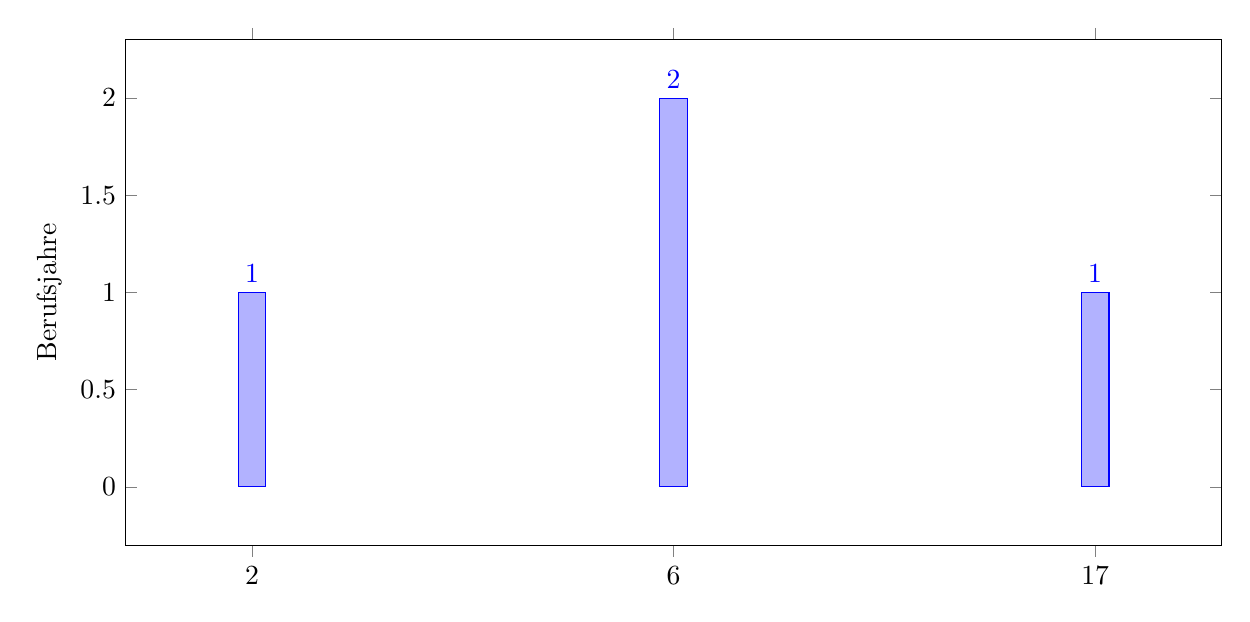
\begin{tikzpicture}
            \begin{axis}[
                ybar, height=8cm, width=15.5cm,
                enlargelimits=0.15,
                legend style={at={(0.5,-0.15)},
                  anchor=north,legend columns=-1},
                ylabel={Berufsjahre},
                ymin=0, ymax=2,
                symbolic x coords={2, 6, 17},
                xtick=data,
                nodes near coords,
                nodes near coords align={vertical},
                ]
            \addplot coordinates {
                (2, 1) 
                (6, 2) 
                (17, 1)
                };
            \end{axis}
        \end{tikzpicture}
        \caption{Berufsjahre der Therapeut/innen}
        \label{fig:therapists-work-years}
    \end{figure}
\fi

% therapists-work-fields
\iffalse
    \begin{figure}[H]
        \centering
        \begin{tikzpicture}
            \pie[pos={10,0}, sum=auto, radius=2, text=legend, color={orange, green, cyan, red}]{50/Psychologie, 25/Klinische Psychologie, 25/Ergotherapie, /Physiotherapie}
        \end{tikzpicture}
        \caption{Aufteilung der Therapeut/innen nach Berufsgruppe}
        \label{fig:therapist-work-fields}
    \end{figure}
\fi
   
In der Abbildung \ref{fig:therapists-school-type} sind die Bildungsgrade der Therapeut/innen dargestellt. Zu den verschiedenen Ausbildungstypen gehört eine Fachhochschule, ein Hochschulstudium sowie ein Masterstudium der Psychologie.

\begin{figure}[H]
    \centering
    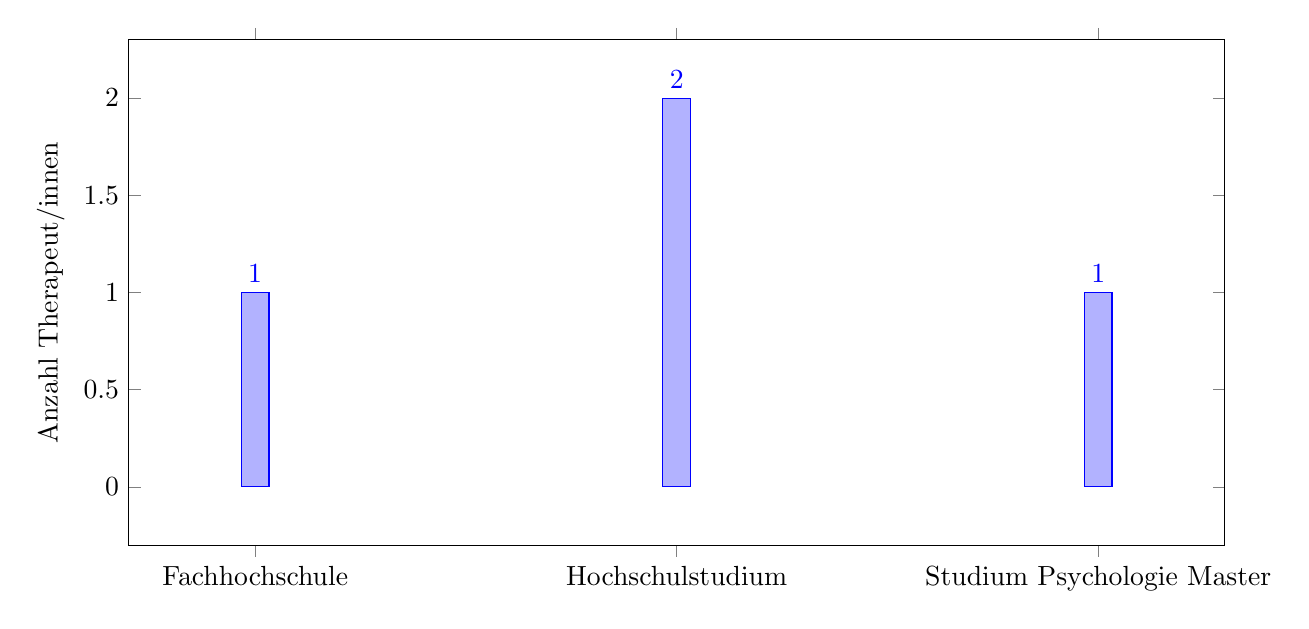
\begin{tikzpicture}
        \begin{axis}[
            ybar, height=8cm, width=15.5cm,
            enlargelimits=0.15,
            legend style={at={(0.5,-0.15)},
              anchor=north,legend columns=-1},
            ylabel={Anzahl Therapeut/innen},
            ymin=0, ymax=2,
            symbolic x coords={Fachhochschule, Hochschulstudium, Studium Psychologie Master},
            xtick=data,
            nodes near coords,
            nodes near coords align={vertical},
            ]
        \addplot coordinates {
            (Fachhochschule, 1) 
            (Hochschulstudium, 2) 
            (Studium Psychologie Master, 1)
            };
        \end{axis}
    \end{tikzpicture}
    \caption{Bildungsgrade der Therapeut/innen}
    \label{fig:therapists-school-type}
\end{figure}

Wie in Abbildung \ref{fig:therapeutic-patient-amount} zu sehen ist, betreuen alle Therapeut/innen zwischen 0 - 50 Patient/innen.

\begin{figure}[H]
    \centering
    \begin{tikzpicture}
        \pie[pos={10,0}, sum=auto, radius=2, text=legend, color={cyan, red, orange, green}]{100/0-50, /51-100, /101-150, /mehr als 150}
    \end{tikzpicture}
    \caption{Wie viele unterschiedliche Patient/innen werden pro Monat betreut?}
    \label{fig:therapeutic-patient-amount}
\end{figure}

Ausnahmslos alle Teilnehmer/innen des Fragebogens setzen Serious Games zur Rehabilitation ein, wie in Abbildung \ref{fig:therapeutic-serious-games-used} zu sehen ist.

\begin{figure}[H]
    \centering
    \begin{tikzpicture}
        \pie[pos={10,0}, sum=auto, radius=2, text=legend, color={cyan, red}]{100/Ja, /Nein}
    \end{tikzpicture}
    \caption{Werden Serious Games zur Rehabiliation eingesetzt?}
    \label{fig:therapeutic-serious-games-used}
\end{figure}

Beim Fragebogen mussten die Teilnehmer/innen angeben, welche Serious Games im LK Allentsteig eingesetzt werden. In Abbildung \ref{fig:therapists-used-serious-games} sind die verschiedenen Spiele dargestellt.  \textit{RehaCom} wird von allen Therapeut/innen verwendet. \textit{CogniPlus} und \textit{FreshMinder} werden von drei Befragten einsetzt. Das Schlusslicht bilden Armeo, Amadeo und MS Kognition, die nur von einer/m Therapeut/in verwendet werden.

\begin{figure}[H]
    \centering
    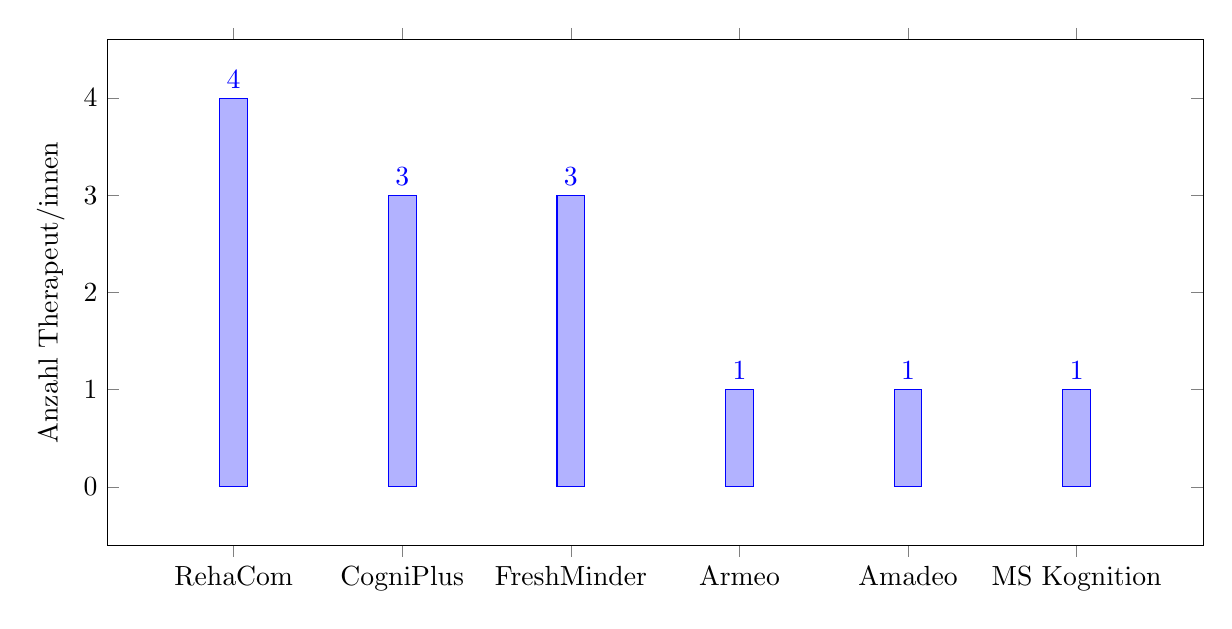
\begin{tikzpicture}
        \begin{axis}[
            ybar, height=8cm, width=15.5cm,
            enlargelimits=0.15,
            legend style={at={(0.5,-0.15)},
              anchor=north,legend columns=-1},
            ylabel={Anzahl Therapeut/innen},
            ymin=0, ymax=4,
            symbolic x coords={RehaCom, CogniPlus, FreshMinder, Armeo, Amadeo, MS Kognition},
            xtick=data,
            nodes near coords,
            nodes near coords align={vertical},
            ]
        \addplot coordinates {
            (RehaCom, 4) 
            (CogniPlus, 3) 
            (FreshMinder, 3)
            (Armeo, 1)
            (Amadeo, 1)
            (MS Kognition, 1)
            };
        \end{axis}
    \end{tikzpicture}
    \caption{Welche Serious Games verwenden Sie?}
    \label{fig:therapists-used-serious-games}
\end{figure}

Danach wurde gefragt, welche Rückmeldung Therapeut/innen von Patient/in beim Einsatz von Serious Games erhalten. Serious Games werden grundsätzlich sehr positiv angenommen, da die Spiele motivierend wirken und die Patient/innen einen Alltagsbezug herstellen können. Allerdings empfinden manche Patient/innen Serious Games als unrealistisch oder nehmen die vorgegebene Reaktionszeit unterschiedlich war. Drei Therapeut/innen geben, dass junge Patient/innen besser auf den Einsatz von Spielen bei der Therapie reagieren. Personen, die sich ihrer kognitiven Schwächen bewusst sind, wollen auch mit Serious Games trainieren.

In Abbildung \ref{fig:therapeutic-where-are-serious-games-used} ist zu sehen, dass 50\% der Patient/innen Serious Games in der Klinik sowohl als auch Zuhause verwenden. Allerdings werden keine Serious Games ausschließlich daheim verwendet.

\begin{figure}[H]
    \centering
    \begin{tikzpicture}
        \pie[pos={10,0}, sum=auto, radius=2, text=legend, color={cyan, orange, red}]{50/Beim Therapeuten vor Ort, 50/Beides, /Zu Hause}
    \end{tikzpicture}
    \caption{Wo verwenden Patient/innen Serious Games?}
    \label{fig:therapeutic-where-are-serious-games-used}
\end{figure}

Um die entwickelte Applikation besser einordnen zu können, wurden weitere Serious Games in die Befragung miteinbezogen. Folgend werden die anderen Serious Games näher erläutert.

\subsubsection{Re@@Ha inkl. RehaLabyrinth}
Re@@Ha ist eine Plattform, welche den Therapeut/innen die Möglichkeit bietet, selbst Serious Games zusammenzustellen. Dadurch können die Spiele an die Patient/innen angepasst werden. Insgesamt sehen die Therapeut/innen diese Funktion positiv, allerdings ist es mit erhöhtem Zeitaufwand verbunden. Bemängelt werden fehlende Erklärungen und die Komplexität der Anwendung.

\subsubsection{MyDailyRoutine}
Dieses Spiel simuliert die Herausforderungen des Alltags und soll die exekutiven Fähigkeiten trainieren. Beispielsweise kann die Zubereitung des Mittagessens simuliert werden. Den Befragten gefällt das Konzept des Spiels besonders gut. Die Therapeut/innen geben an, dass das Spiel viele unterschiedliche neuropsychologische Funktionen trainiert. Des Weiteren wird angemerkt, dass exekutive Funktionen trainiert werden, welche nicht so viele Serious Games bieten. Bemängelt wird die kindliche Darstellung und daraus folgend eine Ablehnung von älteren Personen. Die Therapeut/innen wünschen sich die Implementierung von zusätzlichen Erklärungen und unterschiedliche Schwierigkeitsgrade.

\subsubsection{FoxJump} 
FoxJump ist ein Jump- \& Run-Spiel, welches mithilfe von Handbewegungen gesteuert wird. Im Spiel müssen Objekte eingesammelt werden. Dem/Der Spieler/in stellen sich Gegner in den Weg, denen der/die Patient/in ausweichen soll. Den Befragten gefällt das bunte Farbdesign und der spielerische Charakter des Serious Games. Zwei Personen konnten aufgrund des Videos nicht feststellen, was das genaue Ziel der Anwendung ist. Besonders bemängelt werden die fehlenden Erklärungen und ein veraltetes Design. Bei der Frage, welche Funktionen fehlen wurde angegeben, dass nicht das Gedächtnis oder exekutive Funktionen trainiert werden.

\subsubsection{Reha@Stroke}
Reha@Stroke setzt auf Smartphones und bietet unterschiedliche Interaktionsfunktionen, welche durch die diversen Sensoren und dem Touchscreen der mobilen Geräte ermöglicht werden. Den Therapeut/innen gefällt das einfache, intuitive Design besonders gut. Zudem werden die verschiedenen Schwierigkeitsstufen positiv hervorgehoben. Bemängelt wird die Abstinenz von Erklärungen und Beschriftungen. Als weiteren Kritikpunkt nennen die Therapeut/innen die englische Sprache, die viele Patient/innen nicht verstehen würden. Zudem wird angemerkt die Erforderlichkeit von motorischen Fähigkeiten. Die Therapeut/innen wünschen sich Reaktions- und Gedächtnisaufgaben. Aufgrund des Videos konnte eine Person die benötigte Hardware nicht feststellen.

\subsubsection{Plan your Day}
Diese Anwendung wurde im Verlauf dieser Arbeit erstellt. Das Prinzip des Spiels wird in Abschnitt \ref{sec:iteration1} und \ref{sec:iteration2} näher beschrieben. Den Teilnehmer/innen gefällt der einfache und übersichtliche Aufbau sehr gut. Zudem wird es als alltagsnah und anwendungsbezogen gelobt. Hervorgehoben wurde das Training von exekutiven Funktionen, dem Gedächtnis und der Aufmerksamkeit. Einem/r Teilnehmer/in gefielen die mehreren Planungsschritte. Eine Person bemängelte den Aufbau der Applikation. Verwirrung bei den Therapeut/innen gab es bezüglich der Einordnung von Rezepten zu den Tageszeiten. Teilnehmer/innen merkten an, dass nicht zu viele Aufgaben in die Applikation integriert werden sollen, da Patient/innen damit überfordert werden könnten. Bemängelt wurde das Fehlen eines Schwierigkeitsgrades.

Wie in Abbildung \ref{fig:therapist-game-rating} zu sehen ist, werden die Spiele \textit{Plan your Day} und \textit{MyDailyRoutine} am Besten bewertet. Alle Therapeut/innen würden \textit{Plan your Day} in der Behandlung einsetzen oder zumindest in Betracht ziehen. \textit{MyDailyRoutine} würde von 50\% der Teilnehmer/innen eingesetzt werden. Dreiviertel der Befragten würde \textit{Re@@Ha} vielleicht in der Therapie einsetzen. Bei \textit{FoxJump} und \textit{Re@@Ha} denken 50\% nur über einen Einsatz nach. Die andere Hälfte würde diese beiden Serious Games nicht einsetzen.

\begin{figure}[H]
    \centering
    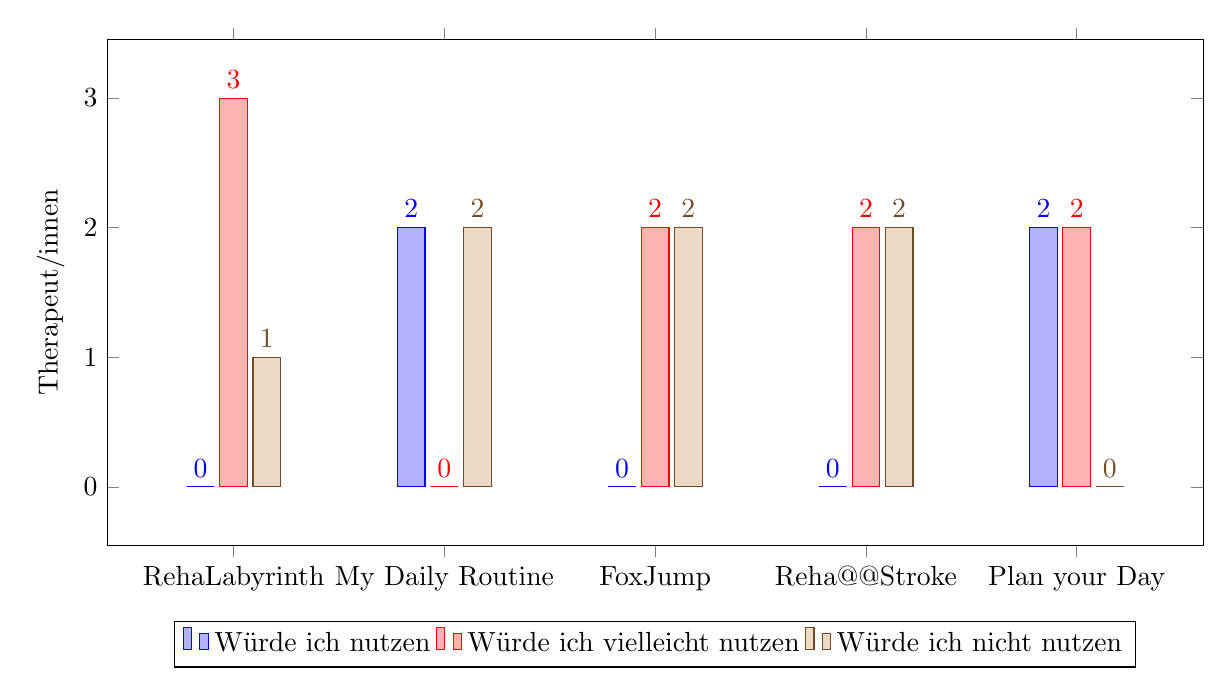
\begin{tikzpicture}
        \begin{axis}[
            ybar, height=8cm, width=15.5cm,
            enlargelimits=0.15,
            legend style={at={(0.5,-0.15)},
              anchor=north,legend columns=-1},
            ylabel={Therapeut/innen},
            ymin=0, ymax=3,
            symbolic x coords={
                RehaLabyrinth, 
                My Daily Routine, 
                FoxJump,
                Reha@@Stroke,
                Plan your Day
            },
            xtick=data,
            nodes near coords,
            nodes near coords align={vertical},
            ]
        \addplot coordinates {
            (RehaLabyrinth, 0) 
            (My Daily Routine, 2) 
            (FoxJump, 0)
            (Reha@@Stroke, 0)
            (Plan your Day, 2)
            };
        \addplot coordinates {
            (RehaLabyrinth, 3) 
            (My Daily Routine, 0) 
            (FoxJump, 2)
            (Reha@@Stroke, 2)
            (Plan your Day, 2)
            };
        \addplot coordinates {
            (RehaLabyrinth, 1) 
            (My Daily Routine, 2) 
            (FoxJump, 2)
            (Reha@@Stroke, 2)
            (Plan your Day, 0)
            };
        \legend{Würde ich nutzen,Würde ich vielleicht nutzen,Würde ich nicht nutzen}
        \end{axis}
    \end{tikzpicture}
    \caption{Bewertung der Serious Games durch Therapeut/innen}
    \label{fig:therapist-game-rating}
\end{figure}

Wie in Abbildung \ref{fig:therapeutic-individual-levels} zu erkennen ist, würden 50\% der Therapeut/innen Serious Games individuell bearbeiten wollen. Kein/e Befragte/r würde das Anpassen von Spielinhalten ablehnen.

\begin{figure}[H]
    \centering
    \begin{tikzpicture}
        \pie[pos={10,0}, sum=auto, radius=2, text=legend, color={cyan, red, orange}]{50/Ja, /Nein, 50/Vielleicht}
    \end{tikzpicture}
    \caption{Würden Sie einzelne Spiellevel individuell selber für den Patienten konfigurieren wollen?}
    \label{fig:therapeutic-individual-levels}
\end{figure}

Die Therapeut/in wollen die Ergebnisse der einzelnen Spielleveln einsehen können, wie in Abbildung \ref{fig:therapeutic-view-results} zu sehen ist. Damit kann der Spielfortschritt von Patient/innen besser beobachtet werden. Aufgrund dieser Daten können die Level schwieriger oder einfacher durch den/die Therapeut/in gestaltet werden.

\begin{figure}[H]
    \centering
    \begin{tikzpicture}
        \pie[pos={10,0}, sum=auto, radius=2, text=legend, color={cyan, red}]{100/Ja, /Nein}
    \end{tikzpicture}
    \caption{Würden Sie Ergebnisse von einzelnen Spiellevel ansehen?}
    \label{fig:therapeutic-view-results}
\end{figure}

\iffalse
    \begin{figure}[H]
        \centering
        \begin{tikzpicture}
            \pie[pos={10,0}, sum=auto, radius=2, text=legend, color={cyan, red, orange}]{100/Ja, /Nein, /Vielleicht}
        \end{tikzpicture}
        \caption{Würden Sie einzelne Spiellevel auf Basis der Ergebnisse adaptieren?}
        \label{fig:therapeutic-adapt-levels}
    \end{figure}
\fi

\iffalse
Am Ende des Fragebogens wurde den Therapeut/innen ein exemplarischer Workflow zur Erstellung von Spielleveln vorgeschlagen. Die Teilnehmer/innen sollten ihre persönliche Meinung äußern und wie gut dieses Konzept in der Therapie angewendet werden kann. In Abbildung \ref{fig:therapeutic-workflow} ist dieser Ablauf dargestellt. Zuerst erstellt oder adaptiert der/die Therapeut/in das Level. Danach wird das Level dem/der gewünschten Patient/in zugewiesen. Der/Die Patient/in spielt daraufhin das Level und Ende werden die Ergebnisse an den/die Therapeut/in übertragen. Die Therapeut/innen gaben an, dass ihrer Meinung nach dieser Workflow bei stationären Patient/innen Wirkung zeigen würde. Jedoch müssen die Ergebnisse der Spielsitzungen nicht sofort übermittelt werden.

\begin{center}
    \smartdiagram[circular diagram:clockwise]{Level/Übung wird von Therapeut/in erstellt/adaptiert, Level/Übung wird von Therapeut/in an Patient/in zugewiesen, Patient/in spielt Spiel, Ergebnisse werden an Therapeut/in übermittelt}
    \captionof{figure}{Workflow zur Erstellung von Levels durch Therapeut/innen}\label{fig:therapeutic-workflow}
\end{center}
\fi

\section{Usability Sicht}
Dieses Unterkapitel definiert den Begriff \enquote{Usability} (deutsch: Gebrauchstauglichkeit). Mit der Gebrauchstauglichkeit im Vordergrund und den speziellen Bedürfnissen der Patient/innen muss die Anwendung zusätzlich angepasst werden. Daher werden die speziellen Designentscheidungen zugunsten der Behandelten beschrieben. Zuletzt wird noch auf die nachträglichen Änderungen eingegangen, die aufgrund von Problemen vorgenommen werden mussten.

\subsection{Usability}
Unter \enquote{Usability} wird oft ein Qualitätsmerkmal für das Entwerfen einer Benutzeroberfläche subsummiert. Zu diesen Merkmalen zählen unter anderem die Anordnung von Bedienelementen, die Anzahl der Klicks um zum Ziel zu gelangen oder die Einfachheit der Anwendung. \cite{richter:2013:usability} \\ 
Der Begriff \enquote{Usability} besteht aus mehreren Komponenten und wird häufig mit diesen fünf Kriterien in Verbindung gebracht: \cite{nielsen:1993:usability}

\begin{itemize}
    \item \textbf{Erlernbarkeit}: Die Einarbeitungszeit der Benutzer/innen in die Anwendung sollte möglichst gering sein.
    \item \textbf{Effizienz}: Das System sollte nach der Einarbeitungsphase sofort nutzbar sein.
    \item \textbf{Einprägsamkeit}: Gelegenheitsbenutzer/innen sollten das System nach längerer Abstinenz problemlos bedienen können, ohne das alles neu gelernt werden muss.
    \item \textbf{Fehler}: Dem/Der Benutzer/in sollten möglichst wenige Fehler bei der Benutzung des Systems unterlaufen. Die gemachten Fehler sollten ohne Probleme korrigierbar sein.
    \item \textbf{Zufriedenheit}: Das System sollte angenehm zu verwenden sein, damit der/die Benutzer/in zufrieden ist.
\end{itemize}

\subsubsection{10 Prinzipien für Interaktions-Design}
\citeauthor{nielsen:1993:usability} hat 1993 10 Prinzipien für gutes Interaktions-Design veröffentlicht. In diesem Abschnitt wird nun näher auf die einzelnen Prinzipien eingegangen, sowie Beispiele zu allen Punkten genannt, die in Zusammenhang mit der entwickelten Applikation stehen.

\paragraph{Simple and natural dialogue}
Dialoge sollen nur Informationen enthalten, die relevant sind. Jede zusätzliche Information steht in Konkurrenz zu anderen und verringert deren Sichtbarkeit. Alle Informationen sollten in einer logischen Reihenfolge sein. \cite{nielsen:1993:usability}

Die Applikation zeigt immer nur eine Information gleichzeitig. Wenn mehrere Meldungen gleichzeitig angezeigt werden, könnte dies den/die Benutzer/in überfordern.

\paragraph{Speek the users' language}
Dialoge sollen in einfachen Worten, Phrasen und Konzepten ausgedrückt werden, die dem/der Benutzer/in bereits bekannt sind. Technische Begriffe, die die meisten Benutzer/innen nicht interpretieren können, sollen nicht verwendet werden. \cite{nielsen:1993:usability}

In Erfolgs- und Fehlermeldungen der Anwendung sind keinerlei technische Begriffe versteckt. Die Hilfetexte sind in natürlicher Sprache verfasst und bieten wenig Interpretationsspielraum.

\paragraph{Minimize the users' memory load}
Benutzer/innen sollen sich nicht unnötig viele Informationen über mehrere Systemschritte merken. Wichtige Hinweise müssen immer sichtbar oder aufrufbar sein. \cite{nielsen:1993:usability}

Jeder Abschnitt des Spiels ist unabhängig voneinander. Der/Die Benutzer/in muss sich außer dem Rezept keinerlei relevante Information merken. Statistiken können im Nachhinein einfach betrachtet werden.

\paragraph{Consistency}
Für den/die Benutzer/in ist es wichtig, dass gewisse Design-Standards eingehalten werden. Gewisse Standards im Design der Oberflächen helfen besser mit dem System zurechtzukommen. Zur Konsistenz gehört auch eine konsistente Benutzer/innenführung. Das bedeutet, dass immer gleiche Begriffe für gleiche Aktionen verwendet werden sollen. \cite{nielsen:1993:usability}

Die Anwendung verwendet ein durchgehend konsistentes Farbdesign. Gewisse Bedienelemente werden immer wieder verwendet, damit sich der/die Benutzer/in einfach zurecht findet.

\paragraph{Feedback}
Der/Die Benutzer/in soll über den aktuellen Systemzustand informiert werden. Direkt nach einer Aktion muss positives oder negatives Feedback zur Situation gegeben werden. \cite{nielsen:1993:usability}

Beispielsweise wird der/die Benutzer/in darauf hingewiesen, dass der jeweilige Spielabschnitt erfolgreich beendet wurde (siehe Abbildung \ref{fig:game-success-message}).

\begin{figure}[H]
    \centering
	\includegraphics[width=0.5\linewidth]{figures/development/application/success-message.png}
	\caption{Erfolgsmeldung, die angezeigt wird, wenn der/die Spieler/in einen Abschnitt erfolgreich absolviert hat.}
	\label{fig:game-success-message}
\end{figure}

\paragraph{Clearly marked exits}
Benutzer/innen passieren immer wieder Fehler, wenn sie in der Applikation navigieren. Dabei soll es möglich sein, dass der/die User/in diesen ungewollten Zustand schnell verlassen kann, ohne dabei unnötig lange aufgehalten zu werden. \cite{nielsen:1993:usability}

Wenn ein/e Benutzer/in eine falsche Option anklickt, dann sollte diese/r nicht die komplette Aktion durchführen müssen, bevor fortgefahren wird. Das Spiel kann zu jeder Zeit abgebrochen werden, wenn es ungewollt gestartet wurde (siehe Abbildung \ref{fig:game-abort-page}).

\begin{figure}[H]
    \centering
    \frame{
	\includegraphics[width=0.4\linewidth]{figures/development/application/abort-message.png}
	}
	\caption{Warnung, die angezeigt wird, wenn der/die Benutzer/in das Spiel vorzeitig verlassen möchte.}
	\label{fig:game-abort-page}
\end{figure}

\paragraph{Shortcuts}
Abkürzungen, die von Anfänger/innen nicht eingesetzt werden, können für Expertenbenutzer/innen einen erheblichen Produktivitätsboost bedeuten. Dadurch ist das System für alle möglichen Benutzer/innengruppen ansprechend. \cite{nielsen:1993:usability}

Ein Beispiel hierfür wären Tastaturshortcuts, die in Textverarbeitungsprogrammen existieren. Die Anwendung erlaubt, dass der Einleitungstext permanent ausgeblendet werden kann (siehe Abbildung \ref{fig:game-introduction-page}). Dazu muss einmalig die Checkbox angeklickt werden. Dies spart erfahrenen Benutzer/innen viel Zeit. Zudem besteht die Möglichkeit diese Einstellung rückgängig zu machen.

\begin{figure}[H]
    \centering
	\includegraphics[width=0.4\linewidth]{figures/development/application/introduction.png}
	\caption{Abschnitt mit dem Einführungstext des Spiels.}
	\label{fig:game-introduction-page}
\end{figure}

\paragraph{Good error messages}
Gute Fehlermeldungen sollen in einfacher Sprache verfasst werden und keine systeminternen Bezeichnungen sein. Das vorliegende Problem muss einfach ausgedrückt und eine Lösung vorschlagen werden. \cite{nielsen:1993:usability}

Dem/Der Benutzer/in sollen keine kryptischen Fehlermeldungen angezeigt werden, die direkt vom System ausgegeben werden, sondern verständliche Fehlerbeschreibungen. In der Anwendung wird dem/der Spieler/in klar mitgeteilt, wodurch der Fehler ausgelöst wurde (siehe Abbildung \ref{fig:game-error-message}).

\begin{figure}[H]
    \centering
	\includegraphics[width=0.5\linewidth]{figures/development/application/error-message.png}
	\caption{Fehlermeldung, die angezeigt wird, wenn der/die Spieler/in eine ungültige Mahlzeit in die Tageszeit \enquote{Frühstück} gezogen hat.}
	\label{fig:game-error-message}
\end{figure}

\paragraph{Prevent errors}
Aussagekräftige Fehlermeldungen sind sehr wichtig, aber noch besser ist, wenn direkt verhindert wird, dass ein Fehler auftritt. Das Design soll es dem/der Benutzer/in erschweren Fehler zu machen. \cite{nielsen:1993:usability}

Dies kann durch den Einsatz einer plattformübergreifenden Designsprache umgesetzt werden. Es existieren einige bekannte Ansätze, etwa das \hyperlink{https://www.microsoft.com/design/fluent/}{Fluent Design} von Microsoft oder das \hyperlink{https://material.io/design/}{Material Design} von Google. Während der Entwicklung wurden die Design-Richtlinien von Google strikt befolgt. 
Laut Google dient das Material Design dazu, dass der verfügbare Platz bestmöglich genutzt wird und ein konsistentes Design auf Smartphones, Tablets und Desktops umgesetzt wird. Das Material Design ist von der physikalischen Welt und deren Texturen inspiriert. Dazu zählt auch wie Licht reflektiert und wie Schatten geworfen werden. \cite{material-design:introduction:2020} \\
Für alle möglichen Komponenten, wie Buttons, Navigationsleisten \acl{usw.}, existieren Best-Practices. Beispielsweise soll eine Top-Bar immer oben sein und dem/der Benutzer/in erlauben, schnell zu navigieren. Der Inhalt darf sich nicht ändern. Dazu existieren noch Empfehlungen in welcher Reihenfolge Symbole in der Leiste angeordnet werden können. Eine Richtlinie ist, dass der Text nicht abgeschnitten werden darf. \cite{material-design:appbar:2020}

\paragraph{Help and documentation}
Am Besten ist, wenn das System ohne Dokumentation verwendbar ist. Trotzdessen sollen Hilfestellungen und Dokumentationen angeboten werden. Diese Informationen müssen einfach zu finden, möglichst kurz und leicht zu verstehen sein. \cite{nielsen:1993:usability}

Der/Die Benutzer/in soll im Falle eines Problems schnell an Hilfe gelangen. In der Anwendung kann der/die User/in in jedem Spielabschnitt den zugehörigen Hilfetext öffnen (siehe Abbildung \ref{fig:game-help-text}). Zudem können alle Zutaten mit Bild außerhalb des Spiels angesehen werden (siehe Abbildung \ref{fig:game-ingredient-info}). Des Weiteren können die Rezepte mit all ihren Bestandteilen, der Schwierigkeit und der Tageszeit angezeigt werden (siehe Abbildung \ref{fig:game-recipe-info}).

\begin{figure}[H]
    \centering
	\includegraphics[width=0.5\linewidth]{figures/development/application/helptext.png}
	\caption{Hilfetext des Spielabschnitts \enquote{Tagesplanung}.}
	\label{fig:game-help-text}
\end{figure}

\begin{figure}[H]
    \centering
	\includegraphics[width=0.5\linewidth]{figures/development/application/ingredient-info.png}
	\caption{Ausschnitt der Überblicksseite über alle Zutaten.}
	\label{fig:game-ingredient-info}
\end{figure}

\begin{figure}[H]
    \centering
	\includegraphics[width=0.35\linewidth]{figures/development/application/recipe-info.png}
	\caption{Ausschnitt der Ansicht, wo alle Rezepte angezeigt werden können. Oben kann zum besseren Überblick nach Tageszeit und Schwierigkeit gefiltert werden.}
	\label{fig:game-recipe-info}
\end{figure}
\section{Architektur}\label{sec:architecture}

Dieses Kapitel beschreibt die Planungsphase des Projekts, sowie die verwendeten Technologien. Dabei wird näher auf die in der Planung verwendeten Strategien eingegangen. Desweiteren werden die wichtigsten Entitäten der Applikation anhand von Diagrammen beschrieben. Danach wird der Architekturstack beschrieben und warum die beschriebenen Tools eingesetzt wurden.

\subsection{Planung}
Dieses Unterkapitel beschäftigt sich mit der theoretischen Planung der Applikation. Es wird auf verschiedene Modellierungssprachen und deren unterschiedliche Diagrammtypen eingegangen. 

\subsubsection{Unified Modeling Language (UML)}
Mithilfe von \acs{UML} können komplexe Sachverhalte aus der Realität verständlich und einfach in Form von mehreren Diagrammtypen dargestellt werden. Durch \acs{UML} können Modelle aus simplen Teilen wie Klassen, Interfaces, Assoziationen, Generalisierungen \ac{usw.} zusammengebaut werden. Um ein komplexes System zu verstehen, muss es aus mehreren Blickwinkeln betrachtet werden. \cite{booch:1999:uml}

\paragraph{Klassendiagramm}
Ein Klassendiagramm stellt ein abstraktes Abbild des Source Codes dar. Es werden Klassen, Interfaces, Methoden und die Beziehung zwischen eben diesen dargestellt. Mit einem Klassendiagramm wird die statische Sicht auf ein System beleuchtet. \cite{booch:1999:uml} \\
Zur besseren Planung wird vor Beginn der Entwicklung ein grobes Konzept der Applikation in Form eines Klassendiagramms entworfen, wodurch die spätere Implementierung für die Entwickler/innen vereinfacht wird. Bereits vor der Implementierung existiert somit ein Grundgerüst, von dem aus der Entwicklungsstart vereinfacht wird. 

\paragraph{Aktivitätsdiagramm}
Ein Aktivitätsdiagramm zeigt den schrittweisen Ablauf von bestimmten Funktionen der Anwendung. Eine Aktivität wird als eine Reihe von Aktionen bezeichnet. Aktionen können verzweigt oder linear ablaufen. Mithilfe von Aktivitätsdiagrammen wird die dynamische Sicht auf ein System dargestellt. \cite{booch:1999:uml} \\
Um die komplexen Abläufe verständlicher darzustellen, werden vor der Implementierung mehrere Aktivitätsdiagramme entworfen. Damit kann auf einen Blick festgestellt werden, welche möglichen Verzweigungen die Funktion aufweist. Anhand des Diagramms können somit auch besser abdeckende Tests entworfen werden. In Abbildung \ref{fig:act-day-planning} ist das Aktivitätsdiagramm des Abschnitts \enquote{Tagesplanung} dargestellt. Der Ablauf der Aktivität wurde bereits im \autoref{chap:day-planning} detailiert beschrieben.

\begin{figure}[H]
    \centering
	\includegraphics[width=0.4\linewidth]{figures/development/planning/activity/day-planning.png}
	\caption{Aktivitätsdiagramm für den Abschnitt \enquote{Tagesplanung}}
	\label{fig:act-day-planning}
\end{figure}

\subsubsection{Entity-Relationship-Modell (ERM)}
Das \acs{ERM} gehört zu den ältesten Modellen zur strukturierten Modellierung von Daten. Eine Klasse in der Objektorientierung entspricht einem Entitätstyp des \acs{ERM}. Entity-Relationship-Diagramme und \acs{UML}-Klassendiagramme haben eine ähnliche Struktur, weswegen \\ \acl{ERM}e auf \acs{UML} abgebildet werden können, jedoch nicht umgekehrt. Der wichtigste Teil des Diagramms sind sogenannte Entitäten, womit Objekte (Gegenstände, Personen, \dots) gemeint sind, die eindeutig identifiziert werden können. Alle Entitäten haben Eigenschaften, denen ein Wertebereich zugeordnet werden kann. Zwischen den Entitäten können unterschiedliche Arten von Beziehungen (1:1, 1:n, n:m) bestehen, die festlegen, wie viele Objekte an einer Beziehung beteiligt sind. \cite{goll:2011:methods_architectures}

Im folgenden Abschnitt wird auf die wichtigsten Teile des finalen \acl{ERM}s eingegangen (siehe Abbildungen \ref{fig:er_users}, \ref{fig:er_recipes}, \ref{fig:er_sessions}). Die unterschiedlichen Entitäten, sowie ihre Beziehungen zueinander werden kurz beschrieben. Um doppelte Formulierungen zu vermeiden werden Attribute, die alle Objekte besitzen nicht beschrieben. Alle Tabellen verfügen über zwei Zeitstempel, die angeben, wann ein Eintrag in die Datenbank eingefügt \acs{bzw.} bearbeitet wurde. Des Weiteren besitzen fast alle Entitäten zur eindeutigen Identifikation eine eindeutige ID.

\begin{figure}[H]
	\includegraphics[width=1\linewidth]{figures/development/planning/er/users.png}
	\caption{Entitäten für die Benutzerverwaltung im \acs{ERM}}
	\label{fig:er_users}
\end{figure}

\paragraph{users}
Zu den zentralen Aspekten der Anwendung zählt die Benutzerverwaltung. Grundsätzlich wird die Applikation von Therapeut/innen und Patient/innen verwendet. Um gemeinsame Funktionen anbieten zu können, fungiert die \textit{users}-Entität als Elterntabelle für die \textit{therapists}- und \textit{patients}-Tabelle. Jede/r User/in kann sich registrieren, anmelden, Passwort zurücksetzen, Profil bearbeiten \acl{usw.}. Spezielle Eigenschaften, welche die Patient/innen und Therapeut/innen haben müssen, werden in den jeweiligen Entitäten beschrieben.

Die wichtigsten Attribute des/der Benutzer/in sind das Passwort und die E-Mail um den Zugang zur Applikation bereitzustellen. Weitere wichtige Attribute sind der Vor- sowie der Nachname und das Geschlecht des/der Anwender/in, damit zwischen den Nutzer/innen unterschieden werden kann. Die Eigenschaften \textit{failed\_login\_attempts} und \textit{login\_cooldown} dienen dazu, dass im Falle eines Missbrauchs des Accounts der/die User/in eine Zeit lang gesperrt werden kann. Die Möglichkeit das Passwort zurückzusetzen, wird durch die Felder \textit{resetcode} und \textit{resetcode\_validuntil} realisiert.

\paragraph{therapists}
Alle Therapeut/innen werden in dieser Tabelle gespeichert. Zusätzlich zu normalen Benutzer/innen müssen Therapeuten nach der Registrierung durch einen Administrator akzeptiert werden (\textit{accepted)}. Anhand der Rolle (\textit{role}) wird festgelegt, ob der Anwender/in ein Admin ist.

\paragraph{patients}
Alle Patienten werden in diesem Objekt abgelegt. Therapierende haben die Möglichkeit weitere Informationen zu den Behandelten zu speichern (\textit{info}), die wiederum von anderen Therapeut/innen abgerufen werden können. Darüber hinaus besitzt der/die Patient/in ein Geburtsdatum, da das Alter für die Therapie relevant sein könnte.

\paragraph{patient\_settings}
Diese Entität beinhaltet Einstellungen, die ein/e Patient/in treffen kann. Die Einstellungen können sich auf das gesamte Spiel auswirken. Dieses Objekt steht in direkter Beziehung (1:1) zum Behandelten.

Die Patient/innen-Einstellungen beinhalten beispielsweise eine Option (\textit{neglect}), ob der/die Betroffene an einem Neglect leidet. Für erfahrene Spieler/innen existiert das Feld \textit{skip\_introduction}, welches erlaubt, dass die Erklärung am Anfang des Spiels übersprungen wird.

\paragraph{therapists\_patients}
Am wichtigsten für die Behandlung ist die Zuweisung von Patient/innen an Therapeut/innen. Die beiden Entitäten (\textit{therapists}, \textit{patients}) sind jeweils mit einer 1:n-Beziehung mit diesem Objekt verbunden. Dies bedeutet, dass ein Therapierender mehrere Patient/innen haben kann und umgekehrt können Behandelte mehrere Therapeut/innen haben.

\begin{figure}[H]
	\includegraphics[width=1\linewidth]{figures/development/planning/er/recipes.png}
	\caption{Entitäten für die Rezeptverwaltung im \acs{ERM}}
	\label{fig:er_recipes}
\end{figure}

\paragraph{recipes}
Zentral für die Applikation sind die unterschiedlichen Rezepte. Diese Rezepte werden in dieser Entität festgehalten. Ein Rezept besitzt einen Namen, sowie eine Beschreibung zur Zubereitung. Zudem verfügt es über eine \textit{Tageszeit} (Frühstück, Mittag- und Abendessen) der Zubereitung und einen \textit{Schwierigskeitsgrad} (Leicht, Mittel, Schwer).
    
\paragraph{ingredients}
Die einzelnen Zutaten der Rezepten werden in der Entität \textit{ingredients} festgehalten. Eine Zutat hat einen \textit{Namen}, ein \textit{Bild} und eine \textit{Lebensmittelkategorie}.
    
\paragraph{recipes\_ingredients}
Die Zuweisung von Rezepten zu Zutaten werden in diesem Objekt festgehalten. Diese Entität steht in einer 1:n-Beziehung mit den Rezepten und Zutaten. Ein Rezept kann mehrere Zutaten haben und eine Zutaten kann in mehreren Rezepten enthalten sein.

\begin{figure}[H]
	\includegraphics[width=1\linewidth]{figures/development/planning/er/sessions.png}
	\caption{Entitäten für die Sitzungsverwaltung im \acs{ERM}}
	\label{fig:er_sessions}
\end{figure}

\paragraph{sessions}
Im Mittelpunk der Applikation stehen die Spielsitzungen. Pro Sitzung werden wichtige Daten gesammelt, die den Therapieerfolg des/der Patient/in über die Zeit widerspiegeln sollen. Jede Session der Spieler/innen wird in der \textit{session}-Enität gespeichert. Die Patient/innen stehen in einer direkten Beziehung (1:1) mit der Session. In derselben Verbindung steht eine Sitzung mit der Entität \textit{Games}. Pro Session existiert eine Statistik.

Das Objekt besitzt noch einen \textit{Zeitpunkt}, an dem die Statistik stattgefunden hat. Dies dient dazu die Sitzung später eindeutig identifizieren zu können.
    
\paragraph{games}
Die verschiedenen Spiele der Applikation werden in dieser Entität abgelegt. Dieses Objekt steht wie oben bereits erwähnt, in einer 1:1 Beziehung mit der Session. Für jedes Spiel existieren mehrere Hilfetexte, daher steht die Entität mit der \textit{helptext\_games}-Entität in einer 1:n Beziehung.

Ein Spiel besitzt einen \textit{Namen} und eine kurze \textit{Beschreibung}. Zudem wird noch der Name der Komponente gespeichert. Dieser Umstand ist nur spiel-intern relevant.
    
\paragraph{statistics}
Die Zeiten pro Spiel und Sitzung werden in dieser Entität abgelegt. Die Statistik steht wie oben bereits beschrieben, in einer 1:1 Verbindung mit der Session. Pro Statistik, können noch mehrere Fehler gespeichert werden, die während des Spiels gemacht wurden. Jene Fehler werden in der Tabelle \textit{errortexts\_statistics} abgelegt.

Eine Statistik besitzt nur einen \textit{Start- und Endzeitpunkt}.
    
\paragraph{texts}
Jeder Abschnitt des Spiels beinhaltet Fehler- sowie Hilfetexte. Diese Texte werden in der \textit{texts}-Entität zusammengefasst. Dieses Objekt dient als übergeordnete Tabelle für \textit{errortexts} und \textit{helptexts}.

Jegliche Form von Text besitzt ein eindeutiges Kürzel (\textit{name}) und den eigentlichen Inhalt (\textit{text}) an sich. 
    
\paragraph{errortexts}
Die Fehlertexte sind eine Spezialisierung der Texte, welche in der Entität \textit{errortexts} zu finden sind. Für alle Arten von Fehlern existiert ein bereits vorgefertigter Text, der dem/der Spieler/in angezeigt wird, sobald diese/r einen Fehler gemacht hat. Das Objekt steht wie oben bereits beschrieben in einer Eltern-Kind Beziehung mit der Entität \textit{texts}.

Ein Fehlertext besitzt zusätzlich noch einen Schweregrad (\textit{severity}) der angibt, wie gravierend der Fehler für das Spiel war.
    
\paragraph{errortexts\_statistics}
Damit die Fehler pro Statistik abgelegt werden können wurde die Entität \textit{errortexts\_statistics} geschaffen. Ein Fehler kann in mehreren Statistiken vorkommen und eine Statistik kann mehrmals den gleichen Fehler haben. Im Nachhinein können sich beide Benutzer/innen-Gruppen alle Fehler mit Text pro Spiel und Sitzung ansehen.
    
\paragraph{helptexts}
Hilfetexte sind eine Ausprägung der Texte, welche in der Entität \textit{helptexts} festgehalten werden. Pro Spiel können mehrere Hilfetexte definiert werden, die dem/der Spieler/in den Einstieg erleichtern sollen, weshalb das Objekt in einer 1:n Verbindung mit der Entität \textit{helptexts\_games} steht. Wie zuvor bereits angemerkt wurde, stehen die Hilfetexte in einer 1:1 Beziehung mit der \textit{texts}-Entität, um auf den Inhalt des Texts zugreifen zu können.
    
\paragraph{helptexts\_games}
Die Zuordnung von Hilfetexten zu Spielen werden in dieser Entität abgelegt. Eine Hilfetext kann in mehreren Spielen vorkommen und ein Spiel kann mehrere Hilfetexte beinhalten, weshalb die \textit{helptexts}- und \textit{games}-Enitäten jeweils in einer 1:n Beziehung mit dem \textit{helptexts\_games} Objekt stehen.


\subsection{Eingesetzte Technologien} \label{sec:technologies}
In dieser Anwendung wird eine App für das mobile \ac{OS} Android implementiert, allerdings wird nicht mit androidspezifischen Werkzeugen entwickelt, sondern mit Webtechnologien. Das Ergebnis kann später einfach auf die gewünschte Zielplattform portiert werden. In diesem Kapitel werden die wichtigsten Technologien kurz vorgestellt. Die Beschreibung ist nicht vollständig, sondern soll lediglich die Kernaspekte der Technologien wiedergeben. Zudem wird kurz erklärt, wofür welche Technologie eingesetzt wird und warum diese genutzt wird. Abbildung \ref{fig:technology_stack} zeigt das Zusammenspiel der Technologien und einen beispielhaften Ablauf der Kommunikation in der Applikation.

\begin{figure}[h]
	\includegraphics[width=1\linewidth]{figures/development/technologies/technologien}
	\caption{Technologiestack}
	\label{fig:technology_stack}
\end{figure}

\subsubsection{JavaScript (JS)} \label{tec:javascript}
\ac{JS} ist eine clientseitige Skriptsprache, die verwendet wird, um dynamische Webseiteninhalte zu erstellen und zu verwalten. \ac{JS} ist schwach typisiert und verfügt über objektorientierte, sowie funktionale Programmierparadigmen. Mittels \ac{DOM} und \ac{JS} kann jedes \acs{HTML}-Element einfach manipuliert werden. Zudem können Events auf Elementen definiert werden, die durch den/die User/in beliebig ausgelöst werden können (z.B. Klicken auf eine Schaltfläche). \cite{morris:javascript:2019} \\
\ac{JS} wurde als primäre Programmiersprache gewählt, da die Technologie mittlerweile beliebter auf \href{https://github.com/}{Github} und \href{https://stackoverflow.com/}{StackOverflow} ist als Java, Python oder PHP, wie in Abbildung \ref{fig:github_ranking_programming_language} gezeigt wird. Damit ist sichergestellt, dass die Sprache genug Unterstützung aus der Community erhält und Fragen schnell und kompetent in Foren beantwortet werden.

\begin{figure}[h]
	\includegraphics[width=1\linewidth]{figures/development/technologies/programming_language_rank}
	\caption{Popularität der bekannte Programmiersprachen \cite{grady:language_popularity:2019}}
	\label{fig:github_ranking_programming_language}
\end{figure}

\paragraph{Typescript (TS)} \label{tec:typescript}
\ac{TS} ist eine Programmiersprache, die von Microsoft im Jahre 2012 veröffentlicht wurde. \ac{TS} bildet eine Obermenge von \ac{JS}, wodurch \ac{TS} alle Funktionen von \ac{JS} besitzt und noch viele weitere, die in der aktuellen Version noch nicht unterstützt werden. Der größte Vorteil von \ac{TS} ist die statische Typsicherheit, wodurch Variablen ein Datentyp zugewiesen werden kann. Beim Kompilieren werden die zugewiesenen Typen überprüft und Fehler ausgegeben, falls eine falsche Zuweisung entdeckt wurde. Somit können bereits viele Bugs ausgeschlossen werden, bevor die Applikation ausgeführt wurde. Außerdem werden von \ac{TS} objektorientierte Programmierparadigmen unterstützt, welche die Entwicklung von größeren Anwendungen erleichtern sollen. \cite{lease:typescript:2019} \\
\ac{TS} wird aufgrund der insgesamt besseren Wartbarkeit und Verständlichkeit des entwickelten Programmcodes in allen Bereichen der Applikation statt \acl{JS} eingesetzt.

\subsubsection{Node.js} \label{tec:nodejs}
Mithilfe von Node.js kann \ac{JS} serverseitig verwendet werden. Bidirektionale Kommunikation von Client und Server wird von Node.js in Form von Websockets unterstützt. Traditionelle Web-Applikationen erlauben nicht, dass der Server mit dem Client interagiert, falls sich Daten im Hintergrund ändern. Hinzukommend erfolgt die Abarbeitung von I/O Operationen asynchron, damit die Programmausführung nicht unnötig lange blockiert wird. \cite{nodejs:2013}

\paragraph{Express.js} \label{tec:expressjs}
Express.js ist ein Framework, welches auf Node.js aufsetzt und viele integrierte Features und Funktionen für die Entwicklung einer flexiblen \ac{API} bereitstellt. Ein Kernaspekt von Express ist die Performance. \cite{express:2019} \\ 
Express wird als Backend eingesetzt, welches die Webanfragen der App bearbeitet und die spielrelevanten Daten formatiert in die Datenbank ablegt. Express wurde aus dem Grund gewählt, damit beide Teile der Applikation (Front- \& Backend) in einer Programmiersprache entwickelt werden, was die Komplexität deutlich verringert, da einzelne Aspekte ohne zusätzlichen Aufwand wiederverwendet werden können.

\subsubsection{Angular} \label{tec:angular}
Angular ist ein Framework für \ac{JS}, mithilfe dessen \ac{SPAs} einfach entwickelt werden können. \ac{SPAs} aktualisieren sich dynamisch, während der/die Benutzer/in mit ihnen interagiert. Dadurch bieten sie eine bessere Erfahrung, da keine langen Wartezeiten durch das Neuladen der Webseite entstehen. Zudem kann der Code in mehrere wiederverwendbare Module unterteilt werden. Die Testbarkeit ist ein zentraler Punkt des Frameworks. Unterstützt werden Unit- und End-to-End Tests. \cite{goel:angular:2019}\cite{krukowski:angular:2019} 

\paragraph{Ionic} \label{tec:ionic}
Ionic ist ein Toolkit, mit dem hochqualitative Apps und Desktopapplikationen anhand von gängigen Webtechnologien (\ac{HTML}, \ac{CSS} und \ac{JS}) entwickelt werden können. Ionic bietet offizielle Unterstützung für \nameref{tec:angular}, allerdings befindet sich der Support für andere \acl{JS}-Frameworks wie Vue oder React in Entwicklung. Ein Ziel des Frameworks ist es, dass der Source Code nur einmal geschrieben werden muss und dann auf allen möglichen Plattformen (iOS, Android, Windows, Linux, \dots) ausgeführt werden kann. Mithilfe von Ionic können auch plattformspezifische Funktionen der verschiedenen \acl{OS}e angesteuert werden, wie das Neigen des Smartphones. \cite{ionic:2019} \\
Der Grund für den Einsatz von Ionic ist, dass das Framework Wert auf Einfachheit legt, weshalb das Erlernen der Kernfunktionalität sehr simpel ist. Hinzu kommt, dass das Framework mit einer Menge vorgefertigter Komponenten ausgeliefert wird, die ohne weitere Konfiguration verwendbar sind, wodurch eine Weboberfläche zusammengestellt werden kann. 

\subsubsection{Android} \label{tec:android}
Android ist ein Linux-basiertes \ac{OS}, welches von Google entwickelt und betreut wird. Hauptsächlich kommt Android auf Smartphones zum Einsatz, jedoch gibt es auch angepasste Versionen für Uhren und Fernseher. Die Software ist mit rund 76\% Verbreitung im Juli 2019 das beliebteste mobile \ac{OS} der Welt.
\cite{android:2019}\cite{android:marketshare:2019} \\
Aufgrund der sehr großen Verbreitung und der Beliebtheit wurde Android als primäres Betriebssystem für die App gewählt. Diese Umstände bieten noch weitere Vorteile, denn das Projekt wird aufgrund der Popularität vermutlich noch lange weitergeführt. Zudem wendet Google immense Ressourcen für die Weiterentwicklung und Verbesserung des Systems auf.

%\begin{figure}[h]
%	\includegraphics[width=1\linewidth]{figures/development/technologies/android_versionverbreitung}
%	\caption{Anteile der verschiedenen Android-Versionen an allen Geräten mit Android OS weltweit im Zeitraum 01. bis 07. Mai 2019 \cite{android:distribution:2019}}
%	\label{fig:android_distribtuon}
%\end{figure}

\subsubsection{MySQL} \label{tec:mysql}
MySQL ist das beliebteste Open Source relationale \ac{DBMS}, welches von der Oracle Corporation entwickelt, vermarktet und gewartet wird \cite{mysql:2019}. Die Technologie MySQL wurde gewählt, da die \ac{DB} einfach aufgesetzt und verwaltet werden kann und eine gute Performance bietet. In der \acl{DB} werden Daten zu den absolvierten Spielen in Kombination mit dem/der Patient/in gespeichert. Diese Ergebnisse können später vom Therapierenden ausgewertet werden. Hier kann die Verbesserung über die Zeit einfach anhand von Diagrammen festgestellt werden. Dadurch sieht der/die Therapeut/in mit dem Patient/innen, wie sich die Rehabilitation über die Zeit entwickelt. So kann auf Schwachpunkte in der Therapie gezielt eingegangen werden.




